\documentclass{article}

\usepackage{amsfonts}
\usepackage{amsmath}
\usepackage{amssymb}
\usepackage{amsthm}
\usepackage{caption}
\usepackage{color}
\usepackage{setspace}
\usepackage{enumerate}
\usepackage{fancyhdr}
\usepackage{fullpage}
\usepackage{hyperref}
\usepackage{graphicx}
\usepackage{latexsym}
\usepackage{listings}
\usepackage{mathrsfs}
\usepackage{natbib}
\usepackage[nottoc]{tocbibind}
\usepackage{url}

\providecommand{\all}{\ \forall \ }
\providecommand{\bs}{\backslash}
\providecommand{\e}{\varepsilon}
\providecommand{\E}{\ \exists \ }
\providecommand{\lm}[2]{\lim_{#1 \rightarrow #2}}
\providecommand{\m}[1]{\mathbb{#1}}
\providecommand{\nv}{{}^{-1}}
\providecommand{\ov}[1]{\overline{#1}}
\providecommand{\p}{\newpage}
\providecommand{\q}{$\quad$ \newline}
\providecommand{\rt}{\rightarrow}
\providecommand{\Rt}{\Rightarrow}
\providecommand{\vc}[1]{\boldsymbol{#1}}
\providecommand{\wh}[1]{\widehat{#1}}

\hypersetup{
    colorlinks,
    citecolor=black,
    filecolor=black,
    linkcolor=black,
    urlcolor=blue
}

\renewcommand{\thesection}{Response to Reviewer \arabic{section}}
\renewcommand{\thesubsection}{\arabic{subsection}}

\date{}
\title{\vspace{2cm} Revision of ``Dispersion Estimation and Its Effect on Test Performance in RNA-seq Data Analysis: A Simulation-Based Comparison of Methods" by William Michael Landau and Peng Liu}


\begin{document}


\maketitle

\paragraph{} \indent The authors wish to thank Academic Editor Lin Chen and the two anonymous referees for their careful review of our paper. We have modified the manuscript to address all comments and suggestions, and we believe this process has resulted in a further improved paper. A point-by-point response to all the comments raised during the review process is provided below. Reviewer comments are italicized. Our response in standard text follows each comment, and important excerpts of the updated manuscript are shown in blue. 

\begin{flushleft}
\newpage

\section*{Journal Requirements}

\emph{When addressing the reviewers comments, please can you address the following journal requirements:}
\begin{enumerate}\item \emph{Please ensure that you refer to Figure 7,8 and 9 in your text as, if accepted, production will need this reference to link the reader to the figure.} \q \q
{\bf Response:} Please find direct references to Figures 7, 8, and 9 at the beginning of the second full paragraph on page 11, also copied below. \q

{\color{blue}Figures 6, 7, 8, 9, 10, and 11 show the relationships between AUC and dispersion estimation method for each test setting and simulation setting.}

\end{enumerate}

\section{}

\subsection{Is the manuscript technically sound, and do the data support the conclusions?}

\emph{This manuscript reviews a few popular dispersion estimation methods and then describes a simulation study that compares them in terms of point estimation and the effect on the performance of tests for differential expression. The manuscript is technically sound.} \q

{\bf Response:} Thank you for reviewing our paper, and we are glad that you think this manuscript is technically sound.

\subsection{Has the statistical analysis been performed appropriately and rigorously?}

\emph{Most of the statistical analysis has been performed appropriately and rigorously. However, I have some comments.}
\begin{enumerate}
\item \emph{On page 9, a receiver operating characteristic (ROC) curve is constructed to evaluate the test performance. The procedure of constructing the ROC curve needs to be specified in more details, so the general reader can understand it. I think that the authors calculated the true positive rate and false positive rate based on each specified significance level, and used a series of the significance levels to get the ROC curve. If my thought is correct, instead of the FPR, the AUCs are more comparable with the same range of the significance levels, which were used to obtain the true positive rate and false positive rate.}
\item \emph{From Figure 6 to Figure 11, the AUC values are very small. The authors need to explain for it.}
\end{enumerate}

{\bf Response:} The updated manuscript explains in more detail the steps for constructing an ROC curve, the role of significance levels in this process, and why our AUC values are so small. Please refer to the last paragraph of page 10 and the first paragraph of page 11, also copied below.


{\color{blue}\paragraph{} \indent  
An ROC curve is a graph of the true positive rate (TPR) of the detection of differentially expressed genes vs the false positive rate (FPR). In practice, we define FPR and TPR to be functions of the significance level, $\alpha$, of the tests for differential expression. Specifically,
   
\begin{align*}
\text{FPR}(\alpha) = \frac{\text{FP}(\alpha)}{\text{EE}} \qquad \text{TPR}(\alpha) = \frac{\text{TP}(\alpha)}{\text{DE}},
\end{align*}
where FP($\alpha$) and TP($\alpha$), respectively, are the numbers of false positive and true positive detections at significance level $\alpha$. Also, EE and DE, respectively, are the true numbers of equivalently expressed and differentially expressed genes. In the pseudo-data, we know that EE is 8000 and DE is 2000. In fact, we know exactly which genes are differentially expressed, so we can calculate FP$(\alpha)$ to be the number of equivalently expressed genes with p-values less than $\alpha$ and TP$(\alpha)$ to be the number of differentially expressed genes with p-values less than $\alpha$. Using a fixed range of $\alpha$ values (the same for all ROC curves in this study), we calculate multiple points of the form, (FPR($\alpha$), TPR($\alpha$)) and plot them on the x-y plane. To compensate for gaps in the x direction of the graph, we interpolate the points with a step function that lies beneath a simple linear interpolation, the latter of which may artificially inflate the AUC heuristic explained below.

\paragraph{} 
In this study, we use the area under each ROC curve (AUC) as a relative measure of the quality of a test, where a high AUC indicates relatively good test performance. Here, each AUC is computed only for FPR $< 0.1$ so that testing situations are evaluated only at reasonable significance levels. Please note that AUC not only depends on the quality of a test, but also on the magnitude of differential expression. In Figures 6 through 11, the AUC values are small because in our simulations, the true log fold changes, $\delta_g$, were taken from a standard normal distribution. As a result, the magnitude of differential expression was small for a significant fraction of truly differentially expressed genes.} \q

When you say, ``instead of the FPR, the AUCs are more comparable with the same range of the significance levels", we think that you are suggesting that we plot TPR vs significance level instead of plotting TPR vs FPR. We maintain that plotting TPR vs FPR is reasonable. First of all, an ROC curve with TPR plotted against FPR is a standard tool and is widespread in scientific literature, especially in medical studies. As such, we expect some readers to already be familiar with ROC curves. Second,  FPR is the true average Type I error rate. Significance level, in this case, is only an estimate of the Type I error rate, and its estimation error depends on the distribution of the p-values of the equivalently expressed genes. Hence, if we had plotted significance levels on the x-axis, we would have needed to apply an error control procedure to make sure that the AUC values from different ROC curves are comparable. We would have had a similar problem if we had used the false discovery rate (FDR) instead of FPR.


\subsection{Does the manuscript adhere to standards in this field for data availability?}

\emph{(No comments)}

\subsection{Is the manuscript presented in an intelligible fashion and written in standard English?}

\emph{This manuscript is well-written. I have only one comment. In the third paragraph of page 8, the authors mentioned ``which the labels at the bottom of the figure indicate". I think it is better to rephrase as "which are indicated by the labels at the bottom of the figure".} \q

{\bf Response:} We are glad you think that the manuscript is well-written. We have made your suggested change in the updated version.



\subsection{Additional Comments to the Author (optional)}

\emph{(No comments)}

\section{}

\subsection{Is the manuscript technically sound, and do the data support the conclusions?}

\emph{The manuscript evaluated several recent methods on dispersion estimation and their effects on differential expression test methods through thorough simulation. The simulation considered combination of methods and multiple characteristics of data, such as size and level of dispersion. The manuscript included a well-conducted evaluation of the results from mean squared error of estimation, scatter plot comparison of estimated vs. true dispersion, and sensitivity-specificity evaluation of differentially expressed gene identification. The technics are sound, and the results are useful for practice. However, the following suggestions are made for improvement of the manuscript:} 

\begin{enumerate}
\item \emph{The manuscript mentioned similar studies by Wu et al. and Yu et al. Can the author address similarity and difference between the results of this study to those studies?} \q

{\bf Response:} We are glad you asked. We mention these studies mostly for the sake of giving credit to similar work. However, our study is not 100\% comparable with those of Wu et al. and Yu et al. To explain, we added a new paragraph at the end of the Introduction (first full paragraph of page 3), copied below. 

{\color{blue} \paragraph{} \indent Studies by Wu et al. [7] and Yu et al. [8] also include simulation-based comparisons of methods for estimating negative binomial dispersions from RNA-seq. However, the authors of these studies were primarily concerned with inventing and validating their own methods. Since we do not propose any new methods here, our study has less personal bias than otherwise. In addition, our comparison is broader in scope. Only three methods were compared in the article by Wu et al., six were compared in the study by Yu et al., and both studies ignored alternate versions of these methods. On the other hand, we consider alternate versions of five classes of methods (for example, the ``Common", ``Tagwise" and ``Trended" versions of the APL method described later), giving us a total ten methods to compare. Considering alternate versions not only broadens the comparison, but also helps us isolate key features that help the good methods succeed. Lastly, our scheme for simulating datasets from the negative binomial model is based on real data and preserves observed relationships between the dispersions and the gene-specific mean counts. On the other hand, in the study by Wu et al., dispersion parameters were simulated independently from the means. Yu et al. use several simulation schemes and real datasets, but none of their realistic schemes simulates the negative binomial model, and according to Yu et al., the rest favor either sSeq (their method) or DESeq (described later).} \q

In addition, the first full paragraph on page 9 of the revised manuscript compares the results shown in Figure 3 to a similar figure in the paper by Wu et al. The paragraph is copied below.

{\color{blue}\paragraph{} \indent Wu et al. [7] show a similar figure (their Figure 3) for the Tagwise wqCML method (called ``edgeR" in their paper), the DESeq Maximum method, and the DSS method under their two simulation settings. Their figure suggests that under the MSE metric, the DSS method performs better than the Tagwise wqCML method, which in turn performs better than the DESeq Maximum method. Our results from simulation settings II though VI do not contradict this result. However, in simulation setting I, where sample sizes are extremely small, gene-specific mean counts are relatively low, and dispersions are relatively high (see Figure 1), this ranking is reversed.} \q


Figures 4 and 5 present another opportunity to compare our results with those of the Wu paper. The last paragraph beginning on page 9 now reads,

{\color{blue}\paragraph{} \indent Wu et al. [7] show a similar figure (their Figure 1) for the Tagwise wqCML method (called ``edgeR" in their paper), the DESeq Maximum method, and the DSS method. The patterns in their figure approximately agree with our results for simulation settings I through III. However, for simulations IV through VI, our scatterplots of the DSS-estimated dispersions on the true dispersions show a lower truncation that is not present in the figure by Wu et al. The DSS method may shrink dispersions particularly aggressively under these conditions.} \q


Lastly, the third full paragraph on page 11, copied below, gives a comparison with the Yu paper. 

{\color{blue} \paragraph{} \indent Table 2 of the paper by Yu et al. [8] suggests that the Tagwise wqCML method (called ``edgeR" in their paper) and the DESeq dispersion estimation method perform roughly equally well under the AUC metric.  Our results agree, with the exception of the DESeq testing method in simulation settings I through III, where the DESeq dispersion estimation method performs worse than the Tagwise wqCML method.} \q

All other results are not directly comparable. For example, the Wu paper does not use ROC curves, and the Yu paper does not use our MSE metric. \q




\item \emph{The manuscript reviewed multiple normalization methods. Can the author address why the Anders and Huber method was selected for this study, or address the effect of normalization method on the following dispersion estimation and differential expression test?} \q

{\bf Response:} For a justification of our chosen normalization method, please refer to the last paragraph of page 7, copied below. 

{\color{blue} \paragraph{} \indent Our simulation procedure was configured such that within each pseudo-dataset, the library sizes do not vary systematically. So when analyzing the simulated data, it would be reasonable to set all the library-wise normalization factors, $s_i$, equal to 1. However, since practitioners use nontrivial normalization methods in the field, we borrowed a sophisticated normalization method: specifically, the one described by Anders and Huber [5]. As shown in unpublished work by Yanwen Xiong and Peng Liu [20], this popular normalization method performs on par with the ubiquitous 0.75 quantile and TMM methods described in the introduction, sometimes even surpassing these two alternatives. The results presented in this article were obtained using the method by Anders and Huber, and they agree with the results obtained from setting all normalization factors equal to 1.} \q

\item \emph{In the comparison of estimated vs. true dispersions (Figure 4), systematic biases were shown for certain methods. Can the author address reasons for systematic biases, or at least their effects on differential expression test and suggestion for practical use of these methods? It would be great if the author could address both.} \q

{\bf Response:} For part of the answer to your question, please refer to the second full paragraph on page 10, copied below.

{\color{blue}\paragraph{} \indent Figures 4 and 5 show that some methods systematically overestimate low true dispersions and systematically underestimate high true dispersions. This behavior is exactly what we should expect from shrinkage. Intuitively, shrinkage pulls estimates towards some common focal point. As an immediate and important practical consequence for point estimation, low estimates should increase, high estimates should decrease, and the collective scatter of estimates should narrow. The practical consequences of shrinkage for significance testing, however, are not clear from Figures 4 and 5 alone. For real insight into hypothesis testing, we need the results of the next subsection.} \q

In other contexts, shrinkage is usually a form of bias that decreases variance. However, in this manuscript, we cannot actually show bias, and we went to great lengths to avoid using the word, ``bias". In the statistical sense, bias is equal to $E ( \wh{\theta} ) - \theta$ for some estimator $\wh{\theta}$ of a parameter $\theta$, and $\text{Mean Squared Error}(\wh{\theta}) = \text{Variance}(\wh{\theta}) + \text{Bias}(\wh{\theta})^2$. In our case, $\theta$ is a gene-specific dispersion parameter, and we only have one dispersion estimate per gene. With only one observation of $\wh{\theta}$, our estimate of $\text{Variance}(\wh{\theta})$ is always 0 even though we know the variance to be greater than 0. As a result, we cannot separate bias from variance. The best we can do is to calculate mean squared error and display it in Figure 3.


\end{enumerate}
























\subsection{Has the statistical analysis been performed appropriately and rigorously?}

\emph{ The statistical analysis of simulation results are appropriate. The results were evaluated from multiple perspectives as listed in comment to 1, which provided comprehensive information of the results.} \q

\emph{However, the following suggestions are made for improvement of the manuscript:}

\begin{enumerate}
\item \emph{In evaluating the mean squared error through box plot in Figure 3, the author should set the same y-axis scale for the Pickrell pseudo data sets and for the Hammer pseudo data sets, if possible. The current plot has different different scales for the 6 simulation settings, which could be misleading.} \q

{\bf Response:} We have updated Figure 3, shown below. The new version has the same y-axis scale for all boxplots. 

\begin{center}
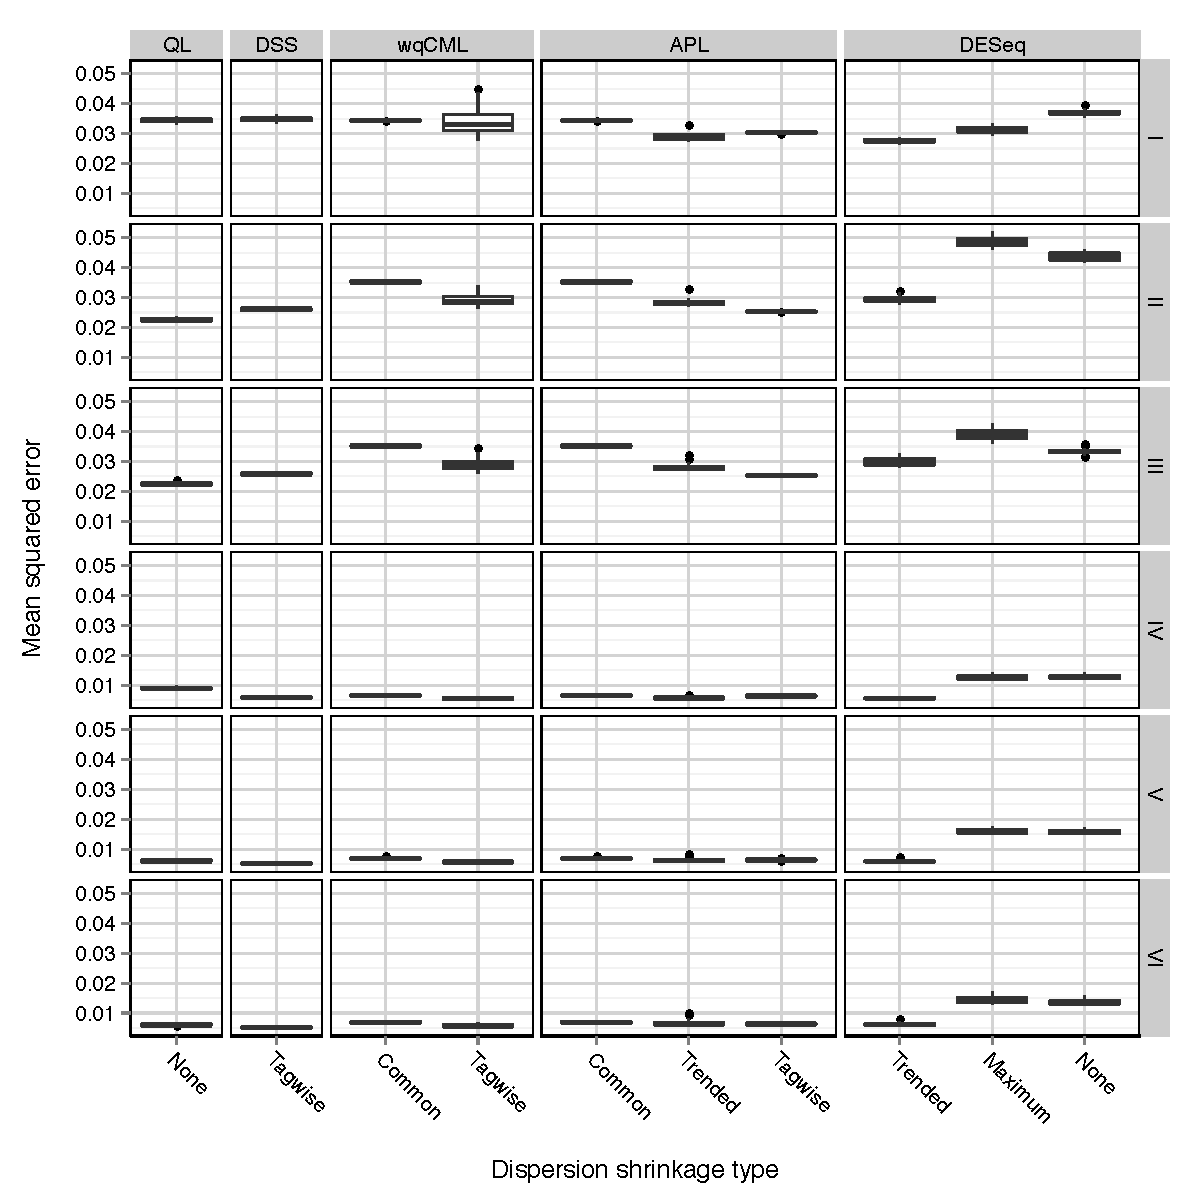
\includegraphics[scale=.5]{../../fig/mse}
\end{center}

\item \emph{Overlapping points between red and green points in Figure 4 are hard to visualize. The author should consider ways of revealing the overlapped points, e.g. by separating the 2 into individual plots, if applicable. This will allow the readers to understand the pattern between estimated and true dispersions through different methods, which is important.} \q

{\bf Response:} We have improved Figures 4 and 5 so that overlapping points are easier to visualize. Previously, there were too many shades of color because we used transparency to indicate both overlap and density. Now, there are only three shades of color: dark blue to indicate overlap, and light blue and black to indicate non-overlapping regions. Below is the new Figure 4.

\begin{center}
 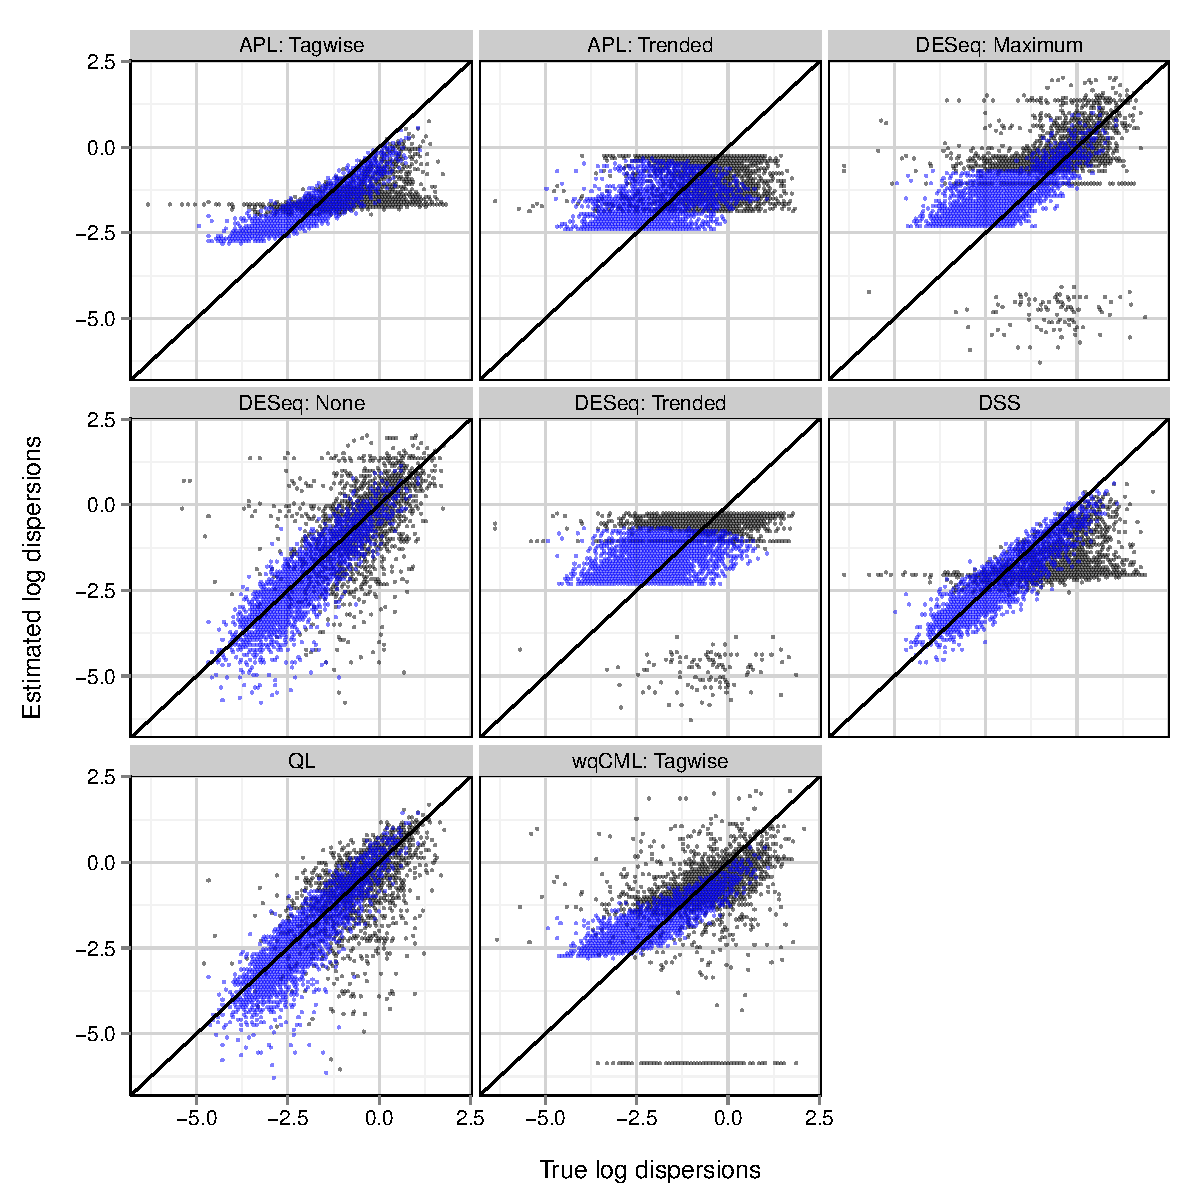
\includegraphics[scale=.5]{../../fig/phi_vs_phi_II_nolegend}
\end{center}

The updated caption reads, \q

{\color{blue} {\bf Simulation setting II: estimated vs true dispersions for an example pseudo-dataset.} Dispersions with gene-wise log geometric mean counts below the median (log mean from $-$2.17 to 1.63) are shown in black %CHANGE: red => black
   , while those above the median (log mean from 1.63 to 10.6) are shown in light blue. %CHANGE: "blue" => "light blue".
   Overlapping points are shown in dark blue. %CHANGE: added "Overlapping points are shown in dark blue." 
   %CHANGE: removed "Bins in these 2D histograms are shaded by log frequency such that a lighter color indicates a lower frequency." 
   Results for simulation settings I and III are similar.} \q
   
Figure 5 and its caption are similar. \q

\item \emph{The manuscript mentioned QL test results as an extreme case, with all dispersion estimation methods showing similar results. Can the author address the reason or any concern for practical application?} \q

{\bf Response:} In the fourth full paragraph on page 11, we now explain why the results of the QL test vary little with the choice of dispersion estimation method, along with some practical consequences. We have included this paragraph below. 

{\color{blue}\paragraph{} \indent Overall, the three tests in the {\tt QuasiSeq} package are less affected by dispersion estimation than the edgeR and DESeq exact tests. These tests introduce gene-wise quasi-likelihood dispersion parameters to the negative binomial model, and the new parameters absorb some of the variability that would otherwise manifest solely in the negative binomial dispersions. The practical upshot is that all three {\tt QuasiSeq} tests are relatively robust under both noisy data and poor estimation of negative binomial dispersions. The QL test is an extreme case, with little change in its AUC boxplots across the dispersion estimation methods, because it does not apply any special constraints to the quasi-likelihood dispersions. (On the other hand, the QLShrink test shrinks the quasi-likelihood dispersions using a common value, and the QLSpline test shrinks them using a fitted spline.) Unfortunately, the QL test also performs the worst among the five tests overall, making it a poor choice in practice despite its otherwise useful robustness. The QLSpline test is better than the QL test, and the QLShrink test is better still.} \q



\item \emph{The manuscript mentioned that Trended APL and Tagwise APL methods yielded similar mean squared errors, but the latter performed better than the former in one test. Can the author provide any insight on the reason?} \q

{\bf Response:} Unfortunately, we have not found a reason why the Tagwise APL method outperforms the Tagwise APL method in significance tests even though the two methods have similar mean squared error. We have added a sentence at the very end of the Discussion section to that effect. The last half of the last full paragraph on page 12 now reads, \q

{\color{blue} In addition, methods with similar MSE may have very different AUC. %CHANGE: "distinct" => "very different"
 For example, the Trended APL and Tagwise APL methods yield similar MSEs in simulation setting V, but the Tagwise APL method performs much better than the Trended APL method in the {\tt edgeR} test (Figure 10). We do not have an explanation for this behavior, but we advise practitioners to think about point estimation and test performance separately when estimating negative binomial dispersions.}


\end{enumerate}










\subsection{Does the manuscript adhere to standards in this field for data availability?}

\emph{This manuscript used simulation data from two real data sets. Access numbers to the real data sets were provided. The simulated data were not deposited for public access.} \q

{\bf Response:} 180 pseudo-datasets were simulated, totaling 46 Mb. Rather than encumber the reader with these files, we elected to submit the 35 kb of computer code needed to reproduce our entire workflow, along with an extensive tutorial and readme. Readers with experience using R and the specified software requirements will be able to generate the pseudo-data for themselves.

\subsection{Is the manuscript presented in an intelligible fashion and written in standard English?}

\emph{The manuscript was very clear and written in standard English. Here are some possible typographical or grammatical issues for the author to check and/or correct:}
\begin{enumerate}
\item \emph{The manuscript used "DE" to stand for "differentially expressed" in some places, but not in others. This should be consistent.}
\item \emph{On page 2, "(TMM) method compute..." should be "(TMM) method computes..."}
\item\emph{ On page 3, the author should check "a real data-based simulation" and see if there is a grammatical error or change the wording to a clearer way.}
\item \emph{On page 3, the "results and discussions sections" should probably be "results and discussion sections" - to be consistent with section titles.}
\item \emph{On page 3, the author should check whether it is appropriate to quote "borrow information across genes" and "shrink".}
\item \emph{On page 5, the author should check "differential expression each gene".}
\item \emph{On page 6, "10000" should be "10,000" to be consistent with others.}
\item \emph{On page 6, in the formula, delta\_h should be delta\_g.}
\item \emph{On page 8, "preform" should be "perform".}
\item \emph{On page 10, "dispersion parameter method" had better be changed to "dispersion estimation method" to be consistent with others.}
\item \emph{On page 10, "a this" should be checked and corrected.}
\end{enumerate}

{\bf Response:} We are glad that you think that the manuscript was clear. All of the above issues are resolved in the updated manuscript, and the changes are tracked in the LaTeX tracked changes file. 

\subsection{Additional Comments to the Author (optional)}

\emph{(No comments)}

\end{flushleft}
\end{document}